\sys introduces a dynamic memory virtualization mechanism that allows tasks to operate primarily through interaction with efficient, volatile SRAM, rather than non-volatile FRAM which, as we showed in Figure~\ref{fig:framEnergy}, is more costly to access than SRAM. \sys supports memory virtualization with a mechanism that moves pages of the address space from their location in a large, non-volatile memory to a small, volatile memory that tasks use during their execution.

\subsection{Paged Non-Volatile Virtual Memory} 

\sys paging scheme partitions the non-volatile memory address space into pages of {\em protected data}. As they are accessed by a task, pages of protected data are swapped into a {\em page buffer} that is stored in volatile memory and holds a single page. When a modified page is swapped out, it is buffered in a dedicated commit buffer for later. \sys uses two-phase commit to write buffered, modified pages back to their original memory locations atomically, ensuring data consistency even with power failures. \sys's page-based memory model allows moving large blocks of data between non-volatile and volatile memory, which \sys does efficiently using common,
hardware DMA block-copy operations, unlike prior work~\cite{chain,alpaca} that moves one variable at a time. Moreover, \sys's paging and buffering scheme is a key enabler of task coalescing, which we describe in Section~\ref{sec:task_coalescing}. Paging simplifies coalescing because deferring a commit of paged data at a task boundary entails leaving paged data buffered only, not requiring additional state management logic at task boundaries.

\subsubsection{Address Translation and Variable Access}

\sys virtualizes the protected, non-volatile data that a task can access through a modified memory interface. The interface includes two operations: \texttt{RVAR(var)}, which reads the value of the memory location {\tt var} and \texttt{WVAR(var,val)}, which writes the value {\tt val} into the memory location {\tt var}. {\tt RVAR} and {\tt WVAR} operations translate a variable's physical address in non-volatile memory and translates it into a \emph{virtual address} in the page buffer \texttt{pageBuf} in volatile memory.  In \sys, a virtual address is composed of a \emph{page tag} and a \emph{page offset}. The page tag identifies in which page of non-volatile memory the memory location resides and the page offset identifies a particular byte of that page. 

%How an $a$-bit memory address decomposes into a tag and an offset depends on the number (and size) of each page of protected memory. To address {\tt p} pages of size {\tt s}, a tag comprises $log(p)$ bits, the offset comprises $log(s)$ bits and $log(p) + log(s) = a$. For example, in a 16-bit address space (i.e., 16\,kB of protected memory) with 512 pages of 128 bytes each, a page's tag is the high-order nine bits of the address and a byte's page offset is the remaining 7 bits.

\begin{algorithm}[t]
	\caption{\texttt{RVAR(var)} pseudo-code}
	\label{algo:rwar}
	\scriptsize
	%\small
	\begin{algorithmic}[1]
		\State $\texttt{tag}\leftarrow \texttt{getTag(var)}$ 
		\If { \texttt{tag} != \texttt{CrntPagTag} }	\Comment{Check if the page is in the page buffer}
		\State	\texttt{PageFault(tag)} \Comment{Page is not in the page buffer, bring it}
		\EndIf
				\State $\texttt{offset}\leftarrow \texttt{getOffset(var)}$ 		
		\State \texttt{return pageBuf[offset]}  \Comment{Return directly from page buffer}
	\end{algorithmic}
\end{algorithm}

After address translation, \sys attempts to access the protected variable's location in the volatile paging buffer. \sys keeps track of the page tag for the page currently resident in the paging buffer in {\tt CrntPagTag}, which is stored in non-volatile memory. When a task accesses a variable, it compares the variable's page tag to {\tt CrntPagTag}.  If an accessed variable's page is equal to {\tt CrntPagTag} then the accessed variable's page is resident in the page buffer. The executing memory operation indexes the page buffer using the variable's page offset and manipulates that byte (i.e., either reading or writing). If the accessed variable's page tag is not equal to {\tt CrntPagTag} then the variable's page is not resident in the page buffer; the operation incurs a {\em page fault}. At a page fault, \sys must swap out the page that is resident in the page buffer and swap in the the variable's page.

Algorithm~\ref{algo:rwar} shows pseudo-code of \texttt{RVAR} and we omit a listing for {\tt WVAR} as it is very similar except it writes the memory location and returns nothing. If the page tag of the variable \texttt{var} and \texttt{CrntPagTag} are not equal (e.g. Lines 2--3), there is a page fault that requires a new page to be swapped in to the page buffer.

\subsubsection{Page Faults and Page Swapping}

\begin{algorithm}[t]
	\caption{\texttt{PageFault(tag)} pseudo-code}
	\label{algo:pagefault}
	\scriptsize
	%\small
	\begin{algorithmic}[1]
		\If {\texttt{isDirty(CrntPagTag)} }	\Comment{Check if the active page is modified}
		\State \texttt{pageCommit(pagesTemp)} \Comment{Phase I commit the active page}
		\EndIf
		\If {\texttt{isDirty(tag)}} \Comment{Check if the requested page has been modified}
		\State {\texttt{getPage(tag,pagesTemp)}=false} \Comment{Get page from the temporary buffer}
		\Else
		\State \texttt{getPage(tag,pagesOrg)}=false \Comment{Get page from the original location}
		\EndIf 
		\State \texttt{CrntPagTag} = \texttt{tag} \Comment{Update tag}
	\end{algorithmic}
\end{algorithm}

A page fault on a memory access requires \sys to swap out whatever page of data is in the page buffer, preserving updates made to that page, and to copy the accessed page of protected data into the page buffer. Algorithm~\ref{algo:pagefault} shows the how \sys handles a page fault. If both the page being swapped out and the page being swapped in are not {\em dirty}---which means that they do not contain bytes modified by the executing task---then handling a page fault simply requires copying the accessed page into the page buffer. If either the {\em resident} page being swapped out or the {\em accessed} page being swapped in is dirty, \sys must take extra steps when handling a page fault. 

\paragraph{Dirty resident page.} If a task modified any byte in the resident page (i.e.,  using \texttt{WVAR}), then the page is dirty. Before swapping in the accessed page, \sys must first preserve the updated values in the dirty page so that they can eventually be committed back to their locations in memory when the task ends. To preserve dirty values, \sys copies the resident page to its dedicated memory region called \texttt{pagesTemp}, which is acts as a double buffer for each page of protected memory. Dirty pages copied into {\tt pagesTemp} during a task remain there until the task completes, at which point \sys commits the modified pages from {\tt pagesTemp} back to memory.  

\paragraph{Dirty accessed page.} If an accessed page is modified, \sys should swap it into the page buffer from its location in {\tt pagesTemp}, rather than swapping it in from its original location in memory. As Algorithm~\ref{algo:pagefault} shows in Line 3, \sys checks if the requested page was previously modified by the executing task. To track whether a page is modified, \sys stores a dirty bit with the page that is set when a task modifies the page. If an accessed page's dirty bit is set, the page must be swapped in from \texttt{pagesTemp} rather than its original memory location (Line 4), furnishing the task with the page's modified values. If the accessed page is not dirty, \sys swaps it in from its original location in memory (Line 6). After swapping the page in, \sys sets \texttt{CrntPagTag} to the tag of the accessed page (Line 7). \sys uses DMA block copies for all page swapping operations, leveraging the efficiency of hardware support.

\subsubsection{Committing a Page}

When a task completes, it must {\em commit} all (dirty) pages stored in \texttt{pagesTemp} back to their original memory locations. \sys maintains a global, non-volatile {\em commit bit} that indicates that a task is committing. The commit bit is set before the first page is committed and the bit is unset after the last page is committed. If power fails during commit, the commit bit remains set and \sys resumes committing before moving on to execute the next task. To commit pages from {\tt pagesTemp}, \sys iterates over the pages' dirty bits and for each page with its dirty bit set, \sys DMA block-copies the page back to its
original memory location, then clears its dirty bit.

\subsection{Paging Example}

Figure~\ref{fig:volatile-buffer} illustrates the execution of a simple task using \sys's paging mechanism. The task manipulates protected variables {\tt x}, {\tt y}, and {\tt z}, which are in the same page. On accessing {\tt x}, its page is swapped into the page buffer. On accessing {\tt y} and {\tt z}, the task need only access the volatile page buffer. The task updates the page, leaving it dirty at the task's completion. When the task completes, \sys first copies the page from the page buffer into the non-volatile {\tt pagesTemp} region before commit. Then, \sys sets the commit bit, atomically commits the page back to its original memory location, and unsets the commit bit.

\begin{figure}[t]
	\centering
	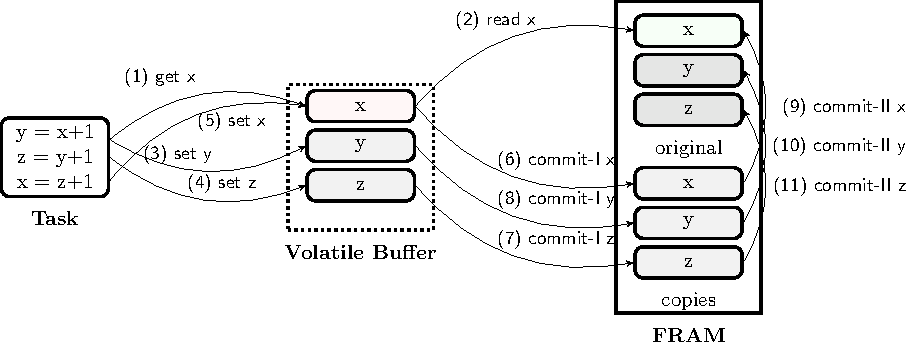
\includegraphics[width=0.75\columnwidth]{figures/sram-buffer}
	\caption{The interaction between the task, volatile buffer and the non-volatile memory (FRAM). Initially, the persistent variable \texttt{x} is not in the volatile buffer but \texttt{y} and \texttt{z} are.}
	\label{fig:volatile-buffer}
\end{figure}

\subsection{Memory Consistency}

\sys's paging mechanism ensures that a task only ever executes using consistent protected data. During task execution, modifications to protected data do not affect their original memory locations because a task reads and writes the volatile page buffer only, and modified pages are swapped out to \texttt{pagesTemp} until commit. A power failure erases the contents of the page buffer, preventing a re-executing task from observing updates in the page buffer from a previous execution attempt. On a reboot after a power failure,
\sys clears all dirty bits in {\tt pagesTemp} {\em if the commit bit is unset}. Clearing these dirty bits ensures that all accesses to protected variables correctly access their original memory locations. The non-volatile commit bit persists across power failures and \sys repeatedly attempts to commit until it succeeds, despite arbitrary power failures.

\subsection{Managing Paging Overhead}

The efficiency of \sys's paging scheme relies on the fact that data in pages are contiguous, which makes them amenable to being manipulated by hardware assisted DMA bulk copy operations. To justify this design choice we experimentally evaluated the efficiency of using DMA block copies, compared to explicit, software copy loops. We copied blocks of data of different size between memory regions on a WISP~\cite{wisp} using a hand-written loop and using DMA (refer to Section~\ref{sec:results_hardware} for hardware setup details). Figure~\ref{fig:dmaTimeEnergy} shows that for moving large blocks of data like a page, hardware DMA is considerably better than software in both run time and energy efficiency. \sys's design moves data in pages, not individual words, leveraging the increased efficiency of DMA data movement.

\begin{figure}[t]
	\centering
	\subfloat[Time needed to transfer a block of data]{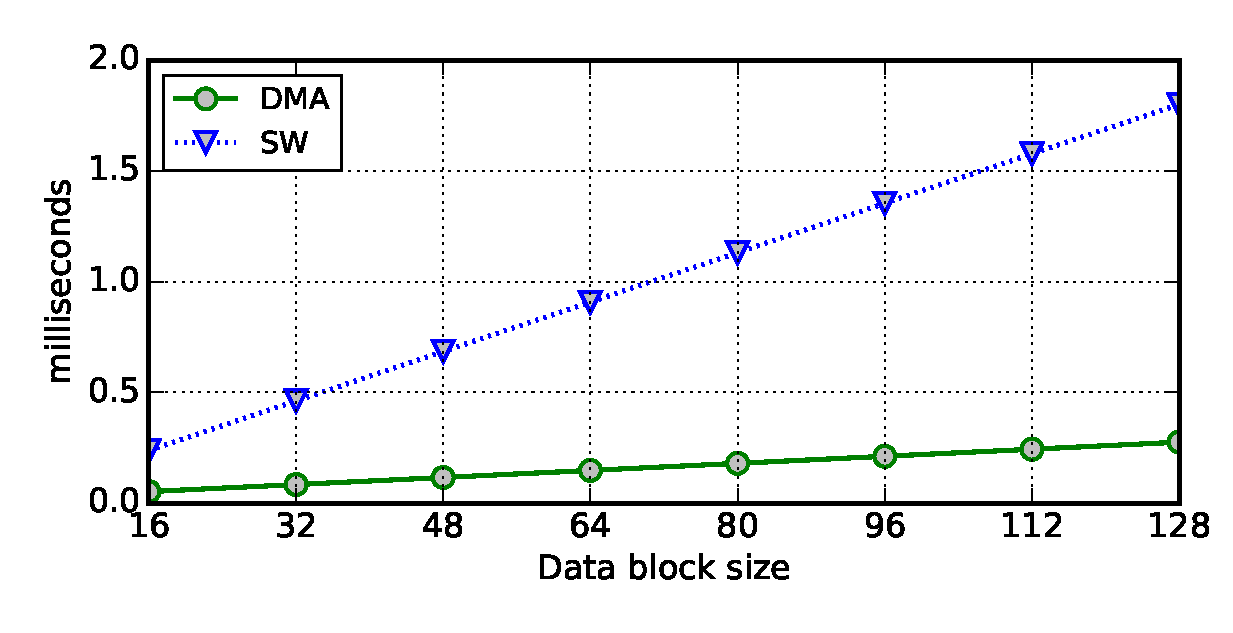
\includegraphics[width=0.49\columnwidth]{figures/dmaSize_time.eps} }
	\subfloat[Energy needed to transfer a block of data]{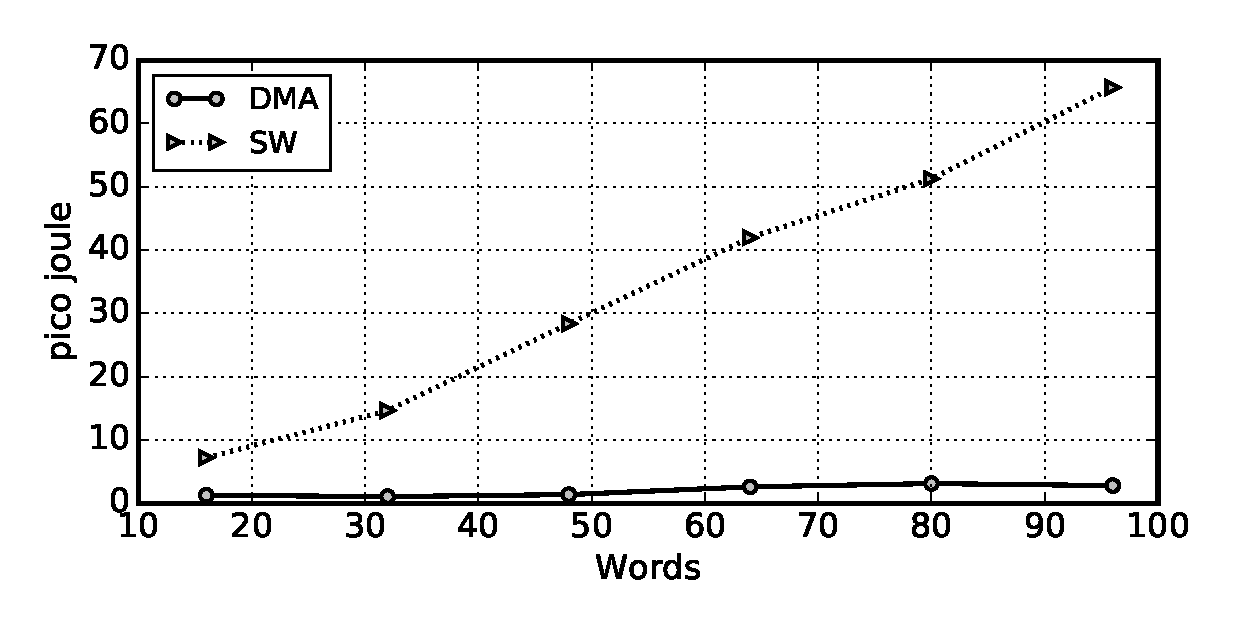
\includegraphics[width=0.49\columnwidth]{figures/energyConsumptionDMA_SW.eps}}
	\caption{Time and energy consumption of moving a block of data from SRAM to FRAM: CPU intervention versus Direct Memory Access (DMA).\todo{Explain HW/SW setup; make fonts larger, unify legends and axes}{Amjad}}
	\label{fig:dmaTimeEnergy}
\end{figure}